\chapter{Introduction}
\label{chp:intro}

We naturally interact with the world and with other human beings by experiencing
multiple senses (\textit{e.g.} sight, hearing, and touch) and using different
communication activities (\textit{e.g.} such as voice, writing, and gestures)
\cite{jaimes_multimodal_2007}. Also, we usually experience those multiple
communication modes simultaneously, and we make sense of the overall environment
through their combination. For instance, during a conversation audio cues allow
us to identify a speaker’s identity and location, while the conversation itself
is commonly extended with gestures.

In contrast with the real complexity of multiple and coordinated interaction
modes we experience in the real world, everyday human–computer interaction still
focuses primarily on a single interaction input mode. Indeed, although everyday
human-computer interaction technologies have supported some forms of multimodal
interaction (\textit{e.g.} by combining text entry, mouse movement and clicks, and by
providing audiovisual output) the model of a single primary channel for data
input, and a single primary channel for data output has been the norm
\cite{turk_multimodal_2014}. Advances in recognition technologies such as
speech, touch, and gesture recognition, however, have given rise to new
human-computer interaction possibilities, such as MUI (Multimodal User
Interfaces) and multiuser interactions.

A MUI~\cite{turk_multimodal_2014} processes two or more combined user input
modalities (\textit{e.g.} speech, pen, touch, gesture, and head and body movements) in a
coordinated manner with output modalities~\cite{oviatt_multimodal_2007}. An
input modality is a mode of
communication~\cite{jaimes_multimodal_2007} that conveys information generated
by human communication activities (\textit{e.g.} speech, gestures) and captured by input
devices (\textit{e.g.} microphone, pen) or sensors (\textit{e.g.} motion sensors). An output
modality is a mode of communication that conveys stimuli to be perceived by the
human senses (\textit{e.g.} hearing, vision). A MUI can uses synthesized audiovisual
content (\textit{e.g.} speech synthesis and avatar) and sensorial effects though
actuators, which can be useful for increasing the
QoE~\cite{ghinea_mulsemedia:_2014}.

\fig{fig:bolt} illustrates Bolt’s seminal work,
“Put-That-There”~\cite{bolt_put-that-there:_1980}, which is an example of
MUI-based interactions.
His system enables users to use gestures and voice commands for planning
tactical activities of military units over a map. The user can move a military
unit by first pointing his/her finger to a unit on the battlefield while saying
“put that”; and then pointing his/her finger to the desired location and saying
“there”. As can be seen in this example, MUIs may support more natural
human-computer interactions since, in many cases, it is possible to emulate the
human-human communication. Bolt’s work also evidences that developing MUIs
brings many new challenges when compared to traditional Graphical User
Interfaces (GUIs). Indeed, when developing MUIs, programmers are required to
handle multiple device configurations and content specifications for both input
and output modalities, as well as the coordination and synchronization among
those modalities.

\begin{figure}[!ht]
\begin{center}
	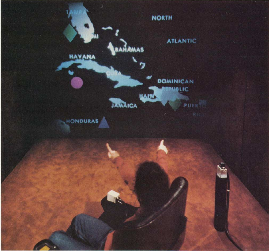
\includegraphics[width=5cm, keepaspectratio]{img/img1.png}
	\caption[Bolt's Put-That-There]{Bolt's Put-That-There from
	~\cite{turk_multimodal_2014}.}
	\label{fig:bolt}
    \captionvspace
\end{center}
\end{figure}

Regarding multiuser interactions, but without considering multimodal features,
some applications can increase the number of interacting users. However,
increasing the number of users does not necessary imply that the system has
become able to identify or distinguish each one of them, \textit{i.e.}~, it does not mean
that the system is fully aware of multiuser interactions. Stefik
~\cite{stefik_wysiwis_1987} proposes the early paradigm of WYSIWIS (What You See
Is What I See). This paradigm enables users to collaborate using the same GUI
across multiple users’ screens. Applications in this paradigm commonly use
shared view tools (\textit{e.g.} VNC--Virtual Network Computing--), and even when multiple users are interacting with
the system, the interacting users are not distinguished and are handled as if they were a single. More recently, research on
Tabletop~\cite{muller-tomfelde_introduction:_2010} and DUI (Distributed
User Interfaces)~\cite{elmqvist_distributed_2011} has been studying multiuser
interaction over shared GUIs, but only few~\cite{dietz_diamondtouch:_2001} of
them truly consider multiuser interactions.

Truly multiuser applications are those in which the system can distinguish, and
the programmer is aware of, the different users who are interacting with the
system~\cite{haber_modeling_2001}. Some authors \cite{laurillau} also call the
interface of
such applications as Identity-aware User interfaces (IAUI). Examples of
application of these truly multiuser interactions are present in gaming and
virtual reality contexts. In these contexts, users are uniquely identified in
each interaction. In game contexts, for instance, users use gamepad or motion
sensors (as illustrated in \fig{fig:multiuser}).

\begin{figure}[!ht]
\begin{center}
	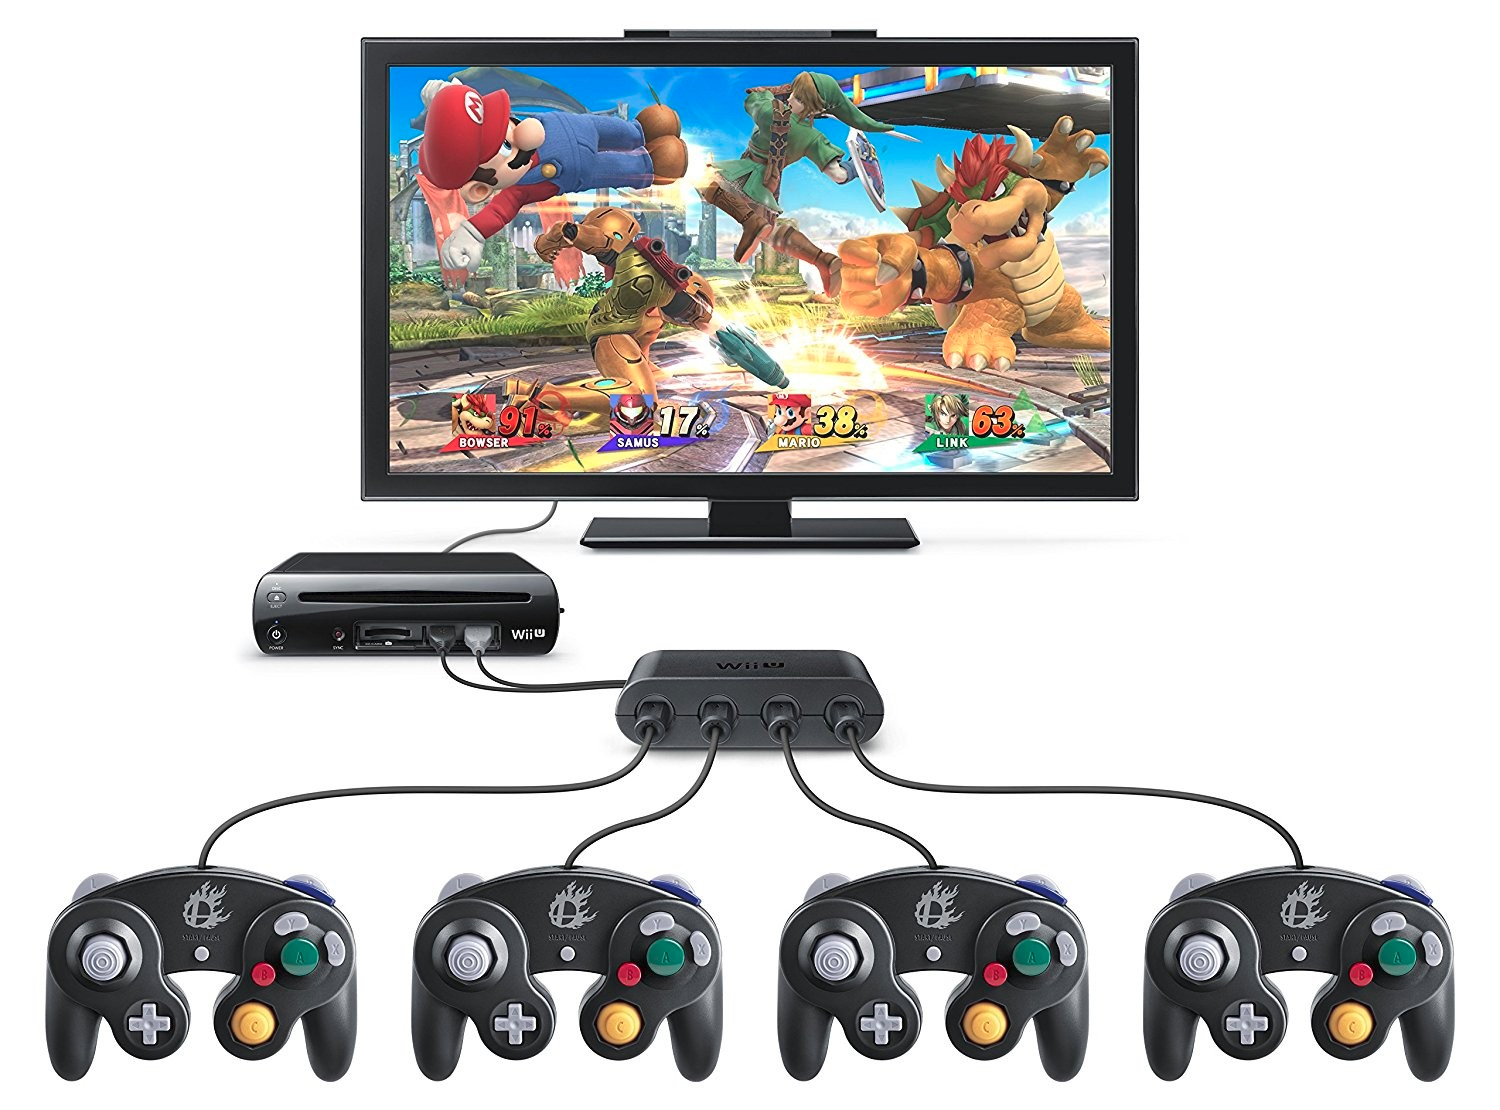
\includegraphics[width=5.5cm, keepaspectratio]{img/img2a.png}
	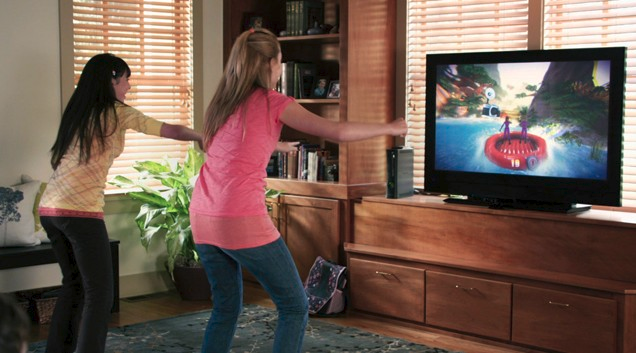
\includegraphics[width=7cm, keepaspectratio]{img/img2b.png}
	\caption[Multiuser games]{Multiuser games with GameCube
	gamepads\footnotemark and Microsoft Kinect\footnotemark}
	\label{fig:multiuser}
    \captionvspace
\end{center}
\end{figure}

\footnotetext[3]{\url{https://images-na.ssl-images-amazon.com/images/I/91Bs1LePe4L._SL1500_.jpg}}
\footnotetext[4]{\url{http://kinectmediaplayerassets.blob.core.windows.net/assets/contexts/adventures/thumb/thumb_kinect_adventures.jpg}}

This thesis addresses development of scenarios that use of human-computer
interaction possibilities, namely MUI and multiuser. To highlight such
scenarios, we present as follows some envisaged ones and their requirements.

\section{Envisaged scenarios and requirements}
\label{sec:intro:scenarios}

Based on Bolt’s scenario, \fig{fig:scenarios} presents the eight envisaged
scenarios of applications that use both multimodal and multiuser interactions.
We organize them by two categories, namely: “Put-That-There”
(\fig{fig:scenarios}-A to D) and “I-Get-That-You-Put-It-There”
(\fig{fig:scenarios}-E to H). Descriptions at the bottom of each scenario follow
the scheme: <number of output modalities, number of input modalities, and number
of interacting users>. We discuss each of them in what follows.

\begin{figure}[!ht]
\begin{center}
    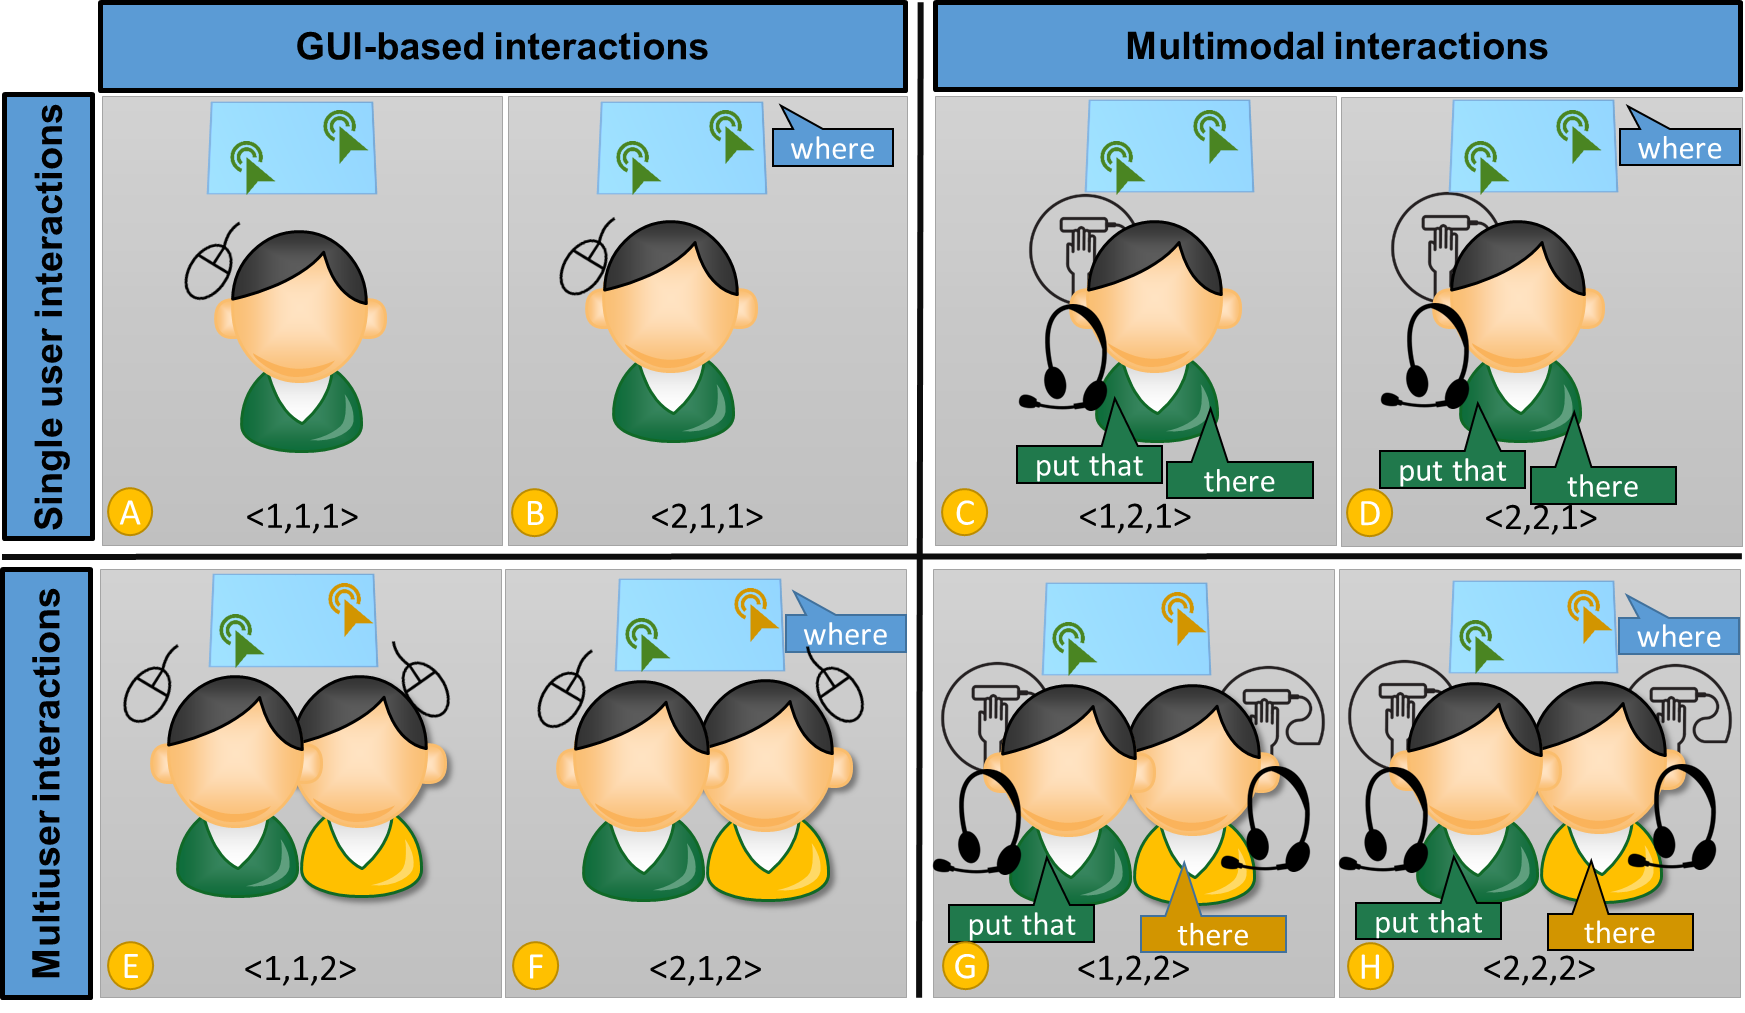
\includegraphics[width=12cm, keepaspectratio]{img/img3.png}
	\caption [Scenarios based on Bolt's Put-that-there]{Scenarios based on
		Bolt's Put-that-there with single/multiple output/input modalities and
		interacting users.}
    \captionvspace
	\label{fig:scenarios}
\end{center}
\end{figure}

The “Put-That-There” category is illustrated in \fig{fig:scenarios}-A to D. It
aims at varying the number of input and/or output modalities for a single user
interacting with the system. While \fig{fig:scenarios}-A and B use GUI-based
interactions, \fig{fig:scenarios}-C and D use multimodal interactions. In
\fig{fig:scenarios}-A, the user interacts using a mouse and gets feedback on a
screen (one input and one output modality). \fig{fig:scenarios}-B extends A with
voice feedback (one additional output modality). In \fig{fig:scenarios}-C, the
user interacts using gestures and voice commands (two input modalities and one
output modality). \fig{fig:scenarios}-D extends C with voice feedback (two input
and two output modalities); it is similar to the original “Put-That-There”. Note
that these scenarios focus on supporting multimodal input/output for a single
user.

The “I-Get-That-You-Put-It-There” category is illustrated in
\fig{fig:scenarios}-E to \fig{fig:scenarios}-H. It is similar to the previous
“Put-That-There”, but the task must be performed by two different users, who are
uniquely identified when interacting with the system. When \fig{fig:scenarios}-E
and \fig{fig:scenarios}-F use GUI-based interactions, \fig{fig:scenarios}-G and
\fig{fig:scenarios}-H use multimodal interactions. \fig{fig:scenarios}-E shows
each user interacting through individual mice. \fig{fig:scenarios}-F extends the
previous one with voice feedback. \fig{fig:scenarios}-G shows each user
interacting through gestures and voice commands. \fig{fig:scenarios}-H extends
the previous one with voice feedback (\textit{i.e.}~, it is similar to the original
“Put-That-There”, but for two users). The “I-Get-That-You-Put-It-There” scenario
can be extended to handle users that are intentionally defined at runtime. For
instance, one may define that the first interaction (\textit{i.e.}~ point and
say “put that”) is carried out by any user and the second interaction
(\textit{i.e.}~ point and say “there”) by a different user. We name this variation as “Anyone-Get-That-Someone-Else-Put-It-There”.

The development of applications for the above scenarios brings both
specification and system requirements.

System must support:

\begin{itemize}
	\item The synchronized presentation of audiovisual media objects. This
	synchronized presentation is required to maintain a coherent visual feedback
	of a MUI-interface;
	\item The presentation of synthesized media objects. MUI interfaces use output
	modalities that are synthesized in presentation time such as synthesized
	audio, avatar or send actions to actuators;
	\item Different input devices. As mentioned, devices such as microphone,
	motion sensors and gamepad may be used by the interacting users;
	\item The matching of the required user characteristics defined by the
	developer with the interacting users. Given the specification of the users
	capable of interacting with application, the system must verify whether a user
	can interact with the application.
\end{itemize}

The specification must support:

\begin{itemize}
	\item Abstractions to use different output and input modalities, besides the
	traditional GUI-based ones. MUI interfaces use output modalities such as:
	synthesized audio, animated avatar, and sensorial effects. Those interfaces
	also use input modalities, such as gesture and speech recognition;
	\item The specification of combined behavior of output and input modalities.
	This support enables the orchestration of both input and output modalities;
	\item Abstractions to define how users should be capable of interacting with
	the application. This support enables the developer to define the
	characteristics users need to have to be able to interact with the
	application. In the Put-That-There scenario, for instance, the developer needs
	to specify that a user needs to have a gesture sensor and a microphone.
\end{itemize}

In this thesis, we focus mainly on the specification requirements above to
define our research goal.

\section{Research goal}
\label{sec:intro:goal}

Given the aforementioned usage scenarios and their specification requirements,
this thesis addresses the following general research question:

\begin{quote}
	\textit{RQ1: How can we support the specification of applications that handle
	both multimodal interactions and multiple interacting users?}
\end{quote}

Some
researches~\cite{dumas_description_2010,katsurada_xisl:_2005,w3c_multimodal_2003}
in Human-Computer Interaction (HCI) also address
this question, but they suffer from some relevant drawbacks (discussed in
\sect{chp:state}). In particular, they lack support for fine synchronization
among modalities. Synchronization among modalities is an issue mainly addressed
by Visualization and Multimedia (VMM) research. Thus, we address this question
by integrating efforts from both HCI and VMM.

In fact, other researchers, such as Rowe~\cite{rowe_looking_2013} and Turk
~\cite{turk_multimodal_2014}, also share our motivation. Rowe’s 2013 ACM SIGMM
Report~\cite{rowe_looking_2013} claimed that multimedia applications with MUI
will be one of main themes for Multimedia research in the next few years.
Additionally, Turk~\cite{turk_multimodal_2014} argued that MUI is a
multidisciplinary object of study. The specification of recognizers and
usability of MUIs are commonly the focus of HCI research, while the
synchronization and development of output modalities are usually the focus of
VMM research. In particularly, VMM research addresses the specification of
synchronization by studies in multimedia languages.

Traditionally, those languages focus on specifying multimedia applications with
synchronized audiovisual media and limited user interactions. Examples of these
languages are: HTML5~\cite{w3c_html_2014}, NCL~(Nested Context Language)~\cite{abnt_abnt_2016}, and SMIL~(Synchronized
Multimedia Integration Language)~\cite{bulterman_smil_2008}. The developer who uses such languages is
usually called author. \fig{fig:overview-multimedia} illustrates an author
creating a multimedia application, and the multimedia system executing it. At
creation time, the author can use abstractions for: media, such as text (\textit{e.g.}~
HTML’s <p>, SMIL’s <text>), graphics (\textit{e.g.} HTML’s <img>), and videos
(\textit{e.g.} HTML’s
<video>); synchronization; and user interactions mainly using mouse
(\textit{e.g.} HTML’s
onClick, NCL’s onSelection) and keyboard (\textit{e.g.} HTML and SMIL’s
keyPress, and
NCL’s onKeySelection). At execution time, the multimedia system presents the
media’s resulting content using audiovisual devices and reacts to pointer and
key-based user interactions.

\begin{figure}[!ht]
\begin{center}
	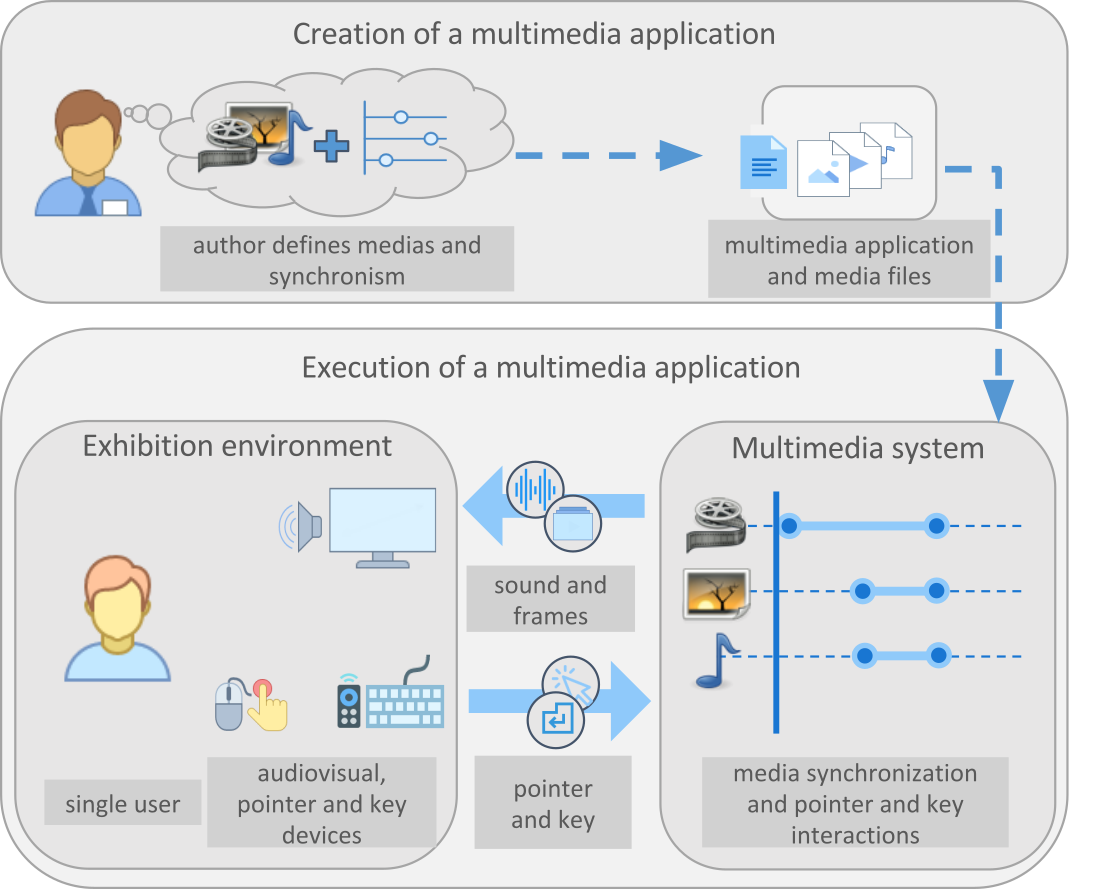
\includegraphics[width=10cm, keepaspectratio]{img/img4.png}
	\caption{Creation and execution of a multimedia application.}
    \captionvspace
	\label{fig:overview-multimedia}
\end{center}
\end{figure}

Given this context of multimedia languages, we argue throughout our research
that the support required by the \textit{RQ1} can be achieved by extending
multimedia languages to support multimodal and multiuser interactions.
Therefore, we define a more specific question to be addressed in this thesis:

\begin{quote}
	\textit{RQ2: How can we extend the output-oriented development in multimedia
	languages to handle multiple modalities of user interactions, besides the
	ordinary GUI-based ones, and multiple interacting users?}
\end{quote}

As discussed in \chp{chp:approach}, our approach proposes extensions to
multimedia languages with first-class entities to support both multimodal and
multiuser features. \fig{fig:overview-multimodal} illustrates our approach as a
new version of the previous figure. At creation time, the author can define not
only the media objects and the synchronization among them, but also the
multimodal and multiuser interactions. For instance, for multimodal
interactions, the author can specify a multimodal description, such as speech
recognition and gesture recognition descriptions. At execution time, the
multimedia system continues to use audiovisual devices to display the content of
the media and pointer/key devices to capture user interactions, but it also uses
multimodal interaction devices. For new output modalities, the multimedia can
also use actuators, which perform sensorial effects, and sensors, which perform
recognitions given multimodal descriptions.

\begin{figure}[!ht]
\begin{center}
	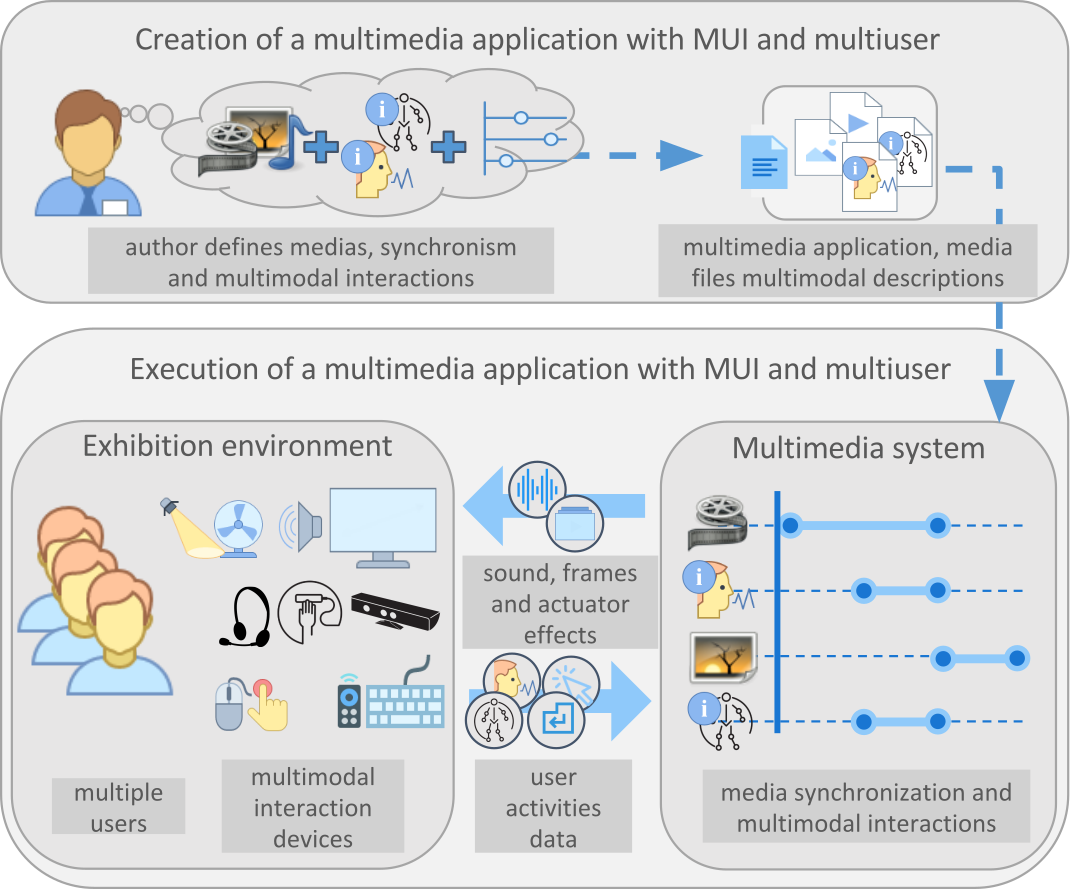
\includegraphics[width=10cm, keepaspectratio]{img/img5.png}
	\caption{Creation and execution of a multimedia application with multimodal
	and multiuser interactions.}
    \captionvspace
	\label{fig:overview-multimodal}
\end{center}
\end{figure}

Some works have aimed at extending multimedia languages (\textit{i.e.}~, those exemplified
in \fig{fig:scenarios}-A to 1-D). However, those works usually add only one new
modality to the language, usually speech
~\cite{beckham_towards_2001,carvalho_architectures_2008,
carvalho_estendendo_2010,	w3c_xhtml+voice_2001,wang_salt:_2002}. The next
chapter briefly discusses those works. To the best of our knowledge, no previous
work has proposed abstractions to support the specification of applications
using both multimodal and multiuser features.

\section{Thesis structure}
\label{sec:intro:structure}

The remainder of this thesis is structured as follows. \chp{chp:state} presents
the related works, languages, and frameworks for the development of multimodal
and multiuser user interfaces, and highlights the main drawbacks of current
approaches. \chp{chp:approach} details our proposed approach to extend
multimedia languages, which overcomes the identified drawbacks.
\chp{chp:instantiation} presents instantiations of the proposed approach in NCL
and HTML languages. \chp{chp:evaluation} presents an evaluation of our proposal.
Finally, \chp{chp:final} presents our final remarks.
